\begin{figure*}[t]
\centering
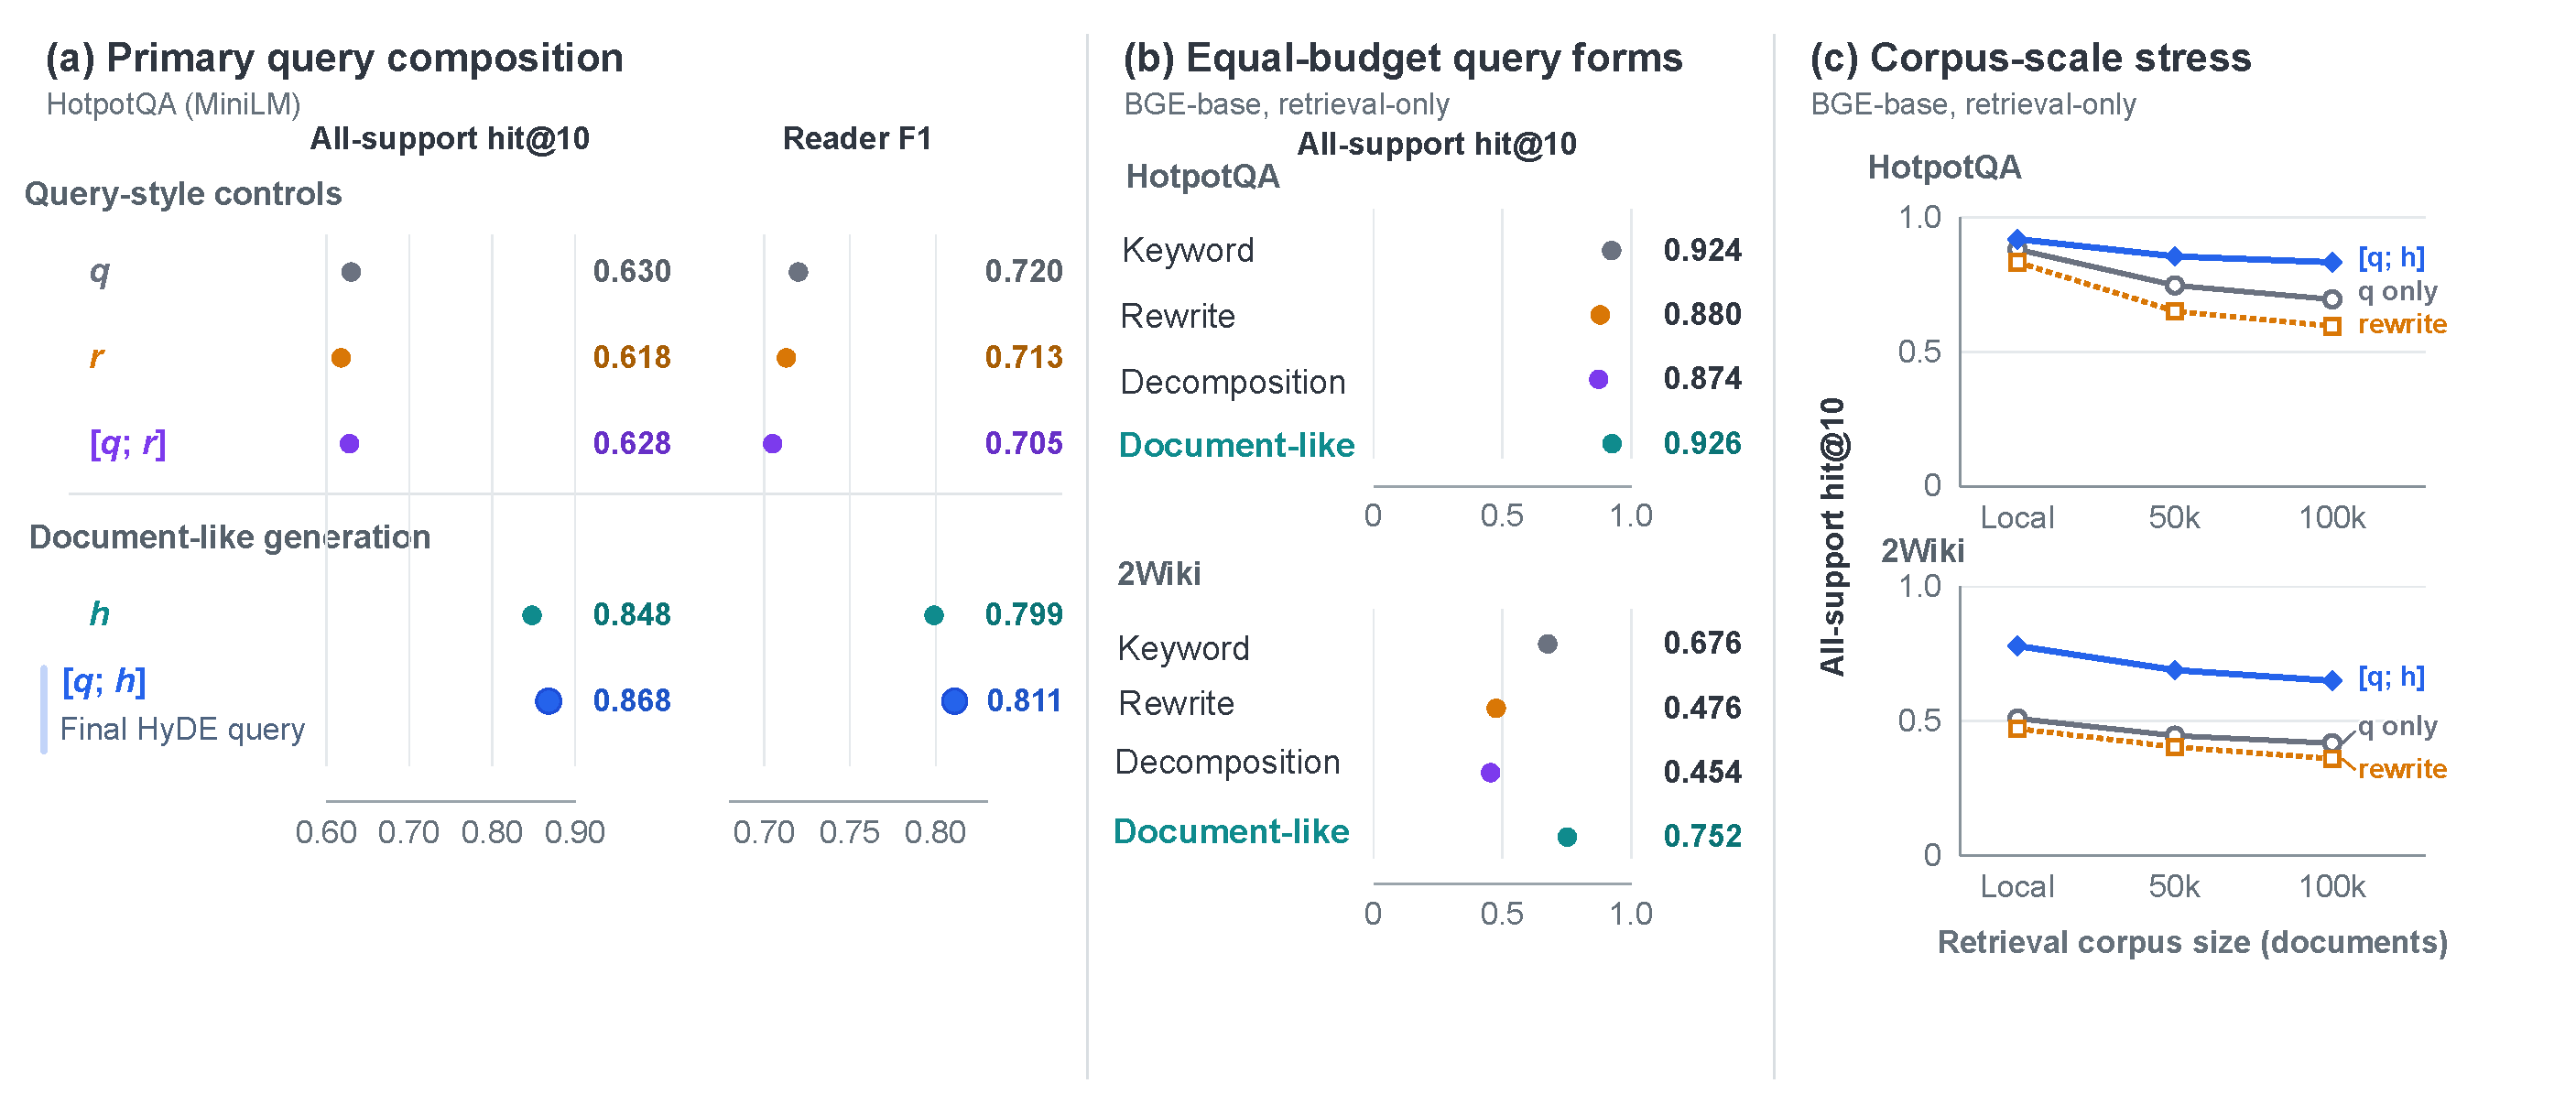
\includegraphics[width=\textwidth]{Fig2.pdf}
\caption{Empirical evidence for HyDE-style query construction. Panel (a) compares primary query compositions on HotpotQA using all-support hit@10 and reader F1. Panel (b) compares equal-budget query forms on HotpotQA and 2WikiMultihopQA. Panel (c) reports all-support hit@10 as the retrieval corpus expands from the original local corpus to 50k and 100k total documents by adding processed-train distractors. Here, $q$ denotes the original question, $r$ a rewritten query, and $h$ a document-like hypothetical passage; $[q; r]$ concatenates the question and rewrite, and $[q; h]$ is the final HyDE query.}
\label{fig:hyde_mechanism_overlap}
\end{figure*}
